% \section{Original data for figure \ref{fig:q1_spatial} \ref{fig:q1_pgd} and \ref{fig:mix_results}}


\section{Omitted experiment results}
\subsection{PTN-ResNet}
\begin{table}[htb]
    \caption{Natural accuracies for training PTN-ResNet18 and PTN-ResNet34 with initial learning rates (lr) = 0.01 or 0.005, trained with different datasets and data augmentations.Each model has four columns of results: ``$D$'' refers to models trained with the natural dataset, while ``$D_R$'' refers to models trained with the robust dataset. The notation $^*$ indicates the model is trained with \texttt{std*} data augmentation. We could not get satisfiable natural accuracy over a reasonable level. Thus, we do not evaluate PTN-ResNet under various spatial attacks and we omit obtained natural accuracy in the main text. We search over initial learning rates {0.01, 0.005} and we log the best results in this table.} \label{tab:ptnresults}
    \begin{adjustwidth}{-.5in}{-.5in}  
        \vspace{15pt}
        \begin{center}
            \begin{tabular}{|c|cccc|cccc|}
                \hline
                  & \multicolumn{4}{c|}{PTN-ResNet18} & \multicolumn{4}{c|}{PTN-ResNet34} \\
         & $D$   & $D_R$        & $D^*$ & $D_R^*$ & $D$          & $D_R$ & $D^*$ & $D_R^*$ \\
         \hline
lr=0.01  & 77.73 & 63.81        & 74.03 & 61.53   & 73.99        & 62.25 & 71.51 & 58.70   \\
lr=0.005 & 77.22 & 66.45        & 75.04 & 62.80   & 74.10        & 61.9  & 70.45 & 58.80  \\
                \hline
            \end{tabular}
        \end{center}
    \end{adjustwidth}
\end{table}

\subsection{STN-ResNet raw experiment results}
\begin{table}[htb]
    \caption{Accuracies achieved with STN-ResNet18 and STN-ResNet34 architectures. The first row of the table contains natural accuracies, while the remaining rows contain robust accuracies under the attack mentioned in the leftmost column. Each model has four columns of results: ``$D$'' refers to models trained with the natural dataset, while ``$D_R$'' refers to models trained with the robust dataset. The notation $^*$ indicates the model is trained with \texttt{std*} data augmentation. We search over initial learning rates {0.01, 0.005} and we log the best results in this table.} \label{tab:stnresults}
    \begin{adjustwidth}{-.5in}{-.5in}  
        \vspace{15pt}
        \begin{center}
            \begin{tabular}{|c|cccc|cccc|}
                \hline
                & 
                % \multicolumn{4}{c|}{ResNet-50} &
                \multicolumn{4}{c|}{STN-ResNet-18} & \multicolumn{4}{c|}{STN-ResNet-34} \\
                Attack & $D$ & $D_R$ & $D^*$ & $D_R^*$ & $D$ & $D_R$ & $D^*$ & $D_R^*$ \\ 
                \hline
                None &
                % 94.84 & 84.75 & 93.9 & 83.53 &  % ResNet-50
                93.55 & 83.75 & 92.83 & 83.05 &  % G-ResNet
                94.05 & 84.39 & 93.12 & 83.72   % STN
                \\
                \texttt{rot10} &
                % 80.97 & 67.78 & 83.24 & 69.67 &  % ResNet-50
                83.54 & 68.66 & 86.46 & 73.08 &  % G-ResNet
                84.07 & 69.52 & 87.67 & 73.55   % STN
                \\
                \texttt{rot30} &
                % 36.77 & 24.94 & 58.75 & 42.62 &  % ResNet-50
                38.66 & 24.98 & 84.72 & 68.93 &  % G-ResNet
                41.01 & 26.4 & 86.1 & 70.86   % STN
                \\
                \texttt{grid775,10$^\circ$} &
                % 63.34 & 52.3 & 67.78 & 55.31 &  % ResNet-50
                68.57 & 54.09 &75.08 &  % G-ResNet
                58.47 & 70.47 & 54.98 & 77.01 & 60.61   % STN
                \\
                \texttt{grid135} &
                % 18.72 & 11.23 & 39.71 & 26.89 &  % ResNet
                20.85 & 11.52 & 65.41 & 49.58 &  % G-ResNet
                22.48 & 11.04 & 69.47 & 50.76   % STN
                \\
                \texttt{grid775} &
                % 15.28 & 9.88 & 35.42 & 24.53 &  % ResNet
                18.22 & 9.9 & 63.48 & 47.49  % G-ResNet
                & 19.94 & 10.09 & 67.47 & 48.64   % STN
                \\
                \hline
            \end{tabular}
        \end{center}
    \end{adjustwidth}
\end{table}

\subsection{G-ResNet raw experiment results}
\begin{table}[htb]
    \caption{Accuracies achieved with G-ResNet18 and G-ResNet34 architectures. The first row of the table contains natural accuracies, while the remaining rows contain robust accuracies under the attack mentioned in the leftmost column. Each model has four columns of results: ``$D$'' refers to models trained with the natural dataset, while ``$D_R$'' refers to models trained with the robust dataset. The notation $^*$ indicates the model is trained with \texttt{std*} data augmentation. We search over initial learning rates {0.1, 0.01}.} \label{tab:spatialattack_g_resnet}
    \begin{adjustwidth}{-.5in}{-.5in}  
        \vspace{15pt}
        \begin{center}
            \begin{tabular}{|c|cccc|cccc|}
                \hline
                & 
                % \multicolumn{4}{c|}{ResNet-50} &
                \multicolumn{4}{c|}{G-ResNet-18} & \multicolumn{4}{c|}{G-ResNet-34} \\
                Attack & $D$ & $D_R$ & $D^*$ & $D_R^*$ & $D$ & $D_R$ & $D^*$ & $D_R^*$ \\ 
                \hline
                None &
                % 94.84 & 84.75 & 93.9 & 83.53 &  % ResNet-50
                94.66 & 85.46 & 94.74 & 85.11 &  % G-ResNet
                \textbf{95.72} & 84.93 & 94.72 & 84.55   % STN
                \\
                \texttt{rot10} &
                % 80.97 & 67.78 & 83.24 & 69.67 &  % ResNet-50
                83.27 & 69.22 & 87.42 & 72.98 &  % G-ResNet
                83.56 & 68.8 & \textbf{87.61} & 73.34   % STN
                \\
                \texttt{rot30} &
                % 36.77 & 24.94 & 58.75 & 42.62 &  % ResNet-50
                41.74 & 26.95 & 69.86 & 51.97 &  % G-ResNet
                41.07 & 26.08 & \textbf{75.38} & 46.47   % STN
                \\
                \texttt{grid775,10$^\circ$} &
                % 63.34 & 52.3 & 67.78 & 55.31 &  % ResNet-50
                68.17 & 54.24 & \textbf{75.7} &  % G-ResNet
                58.96 & 67.98 & 55.15 & \textbf{75.7} & 60.38   % STN
                \\
                \texttt{grid135} &
                % 18.72 & 11.23 & 39.71 & 26.89 &  % ResNet
                21.84 & 11.81 & 52.51 & 36.64 &  % G-ResNet
                20.99 & 10.99 & \textbf{56.06} & 31.52   % STN
                \\
                \texttt{grid775} &
                % 15.28 & 9.88 & 35.42 & 24.53 &  % ResNet
                19.36 & 10.78 & 49.69 & 34.57  % G-ResNet
                & 17.82 & 9.89 & \textbf{53.19} & 29.78   % STN
                \\
                \hline
            \end{tabular}
        \end{center}
    \end{adjustwidth}
\end{table}

\newpage

\begin{figure}[htb]
\section{Training and validation curves while training on $D_{mix}$}
    \vspace{10pt}
    \centering
    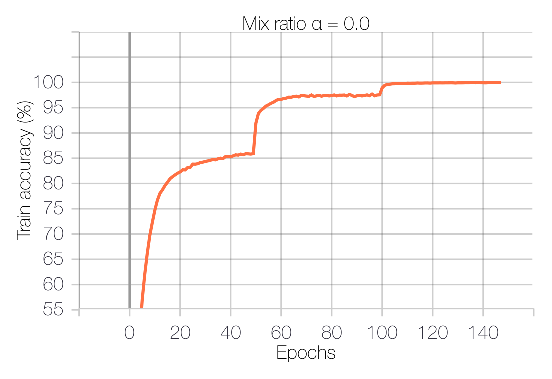
\includegraphics[width=0.48\textwidth]{figs/acc_loss_mix/mix0.0/nat_train_top1.eps}
    \hspace{10pt}
    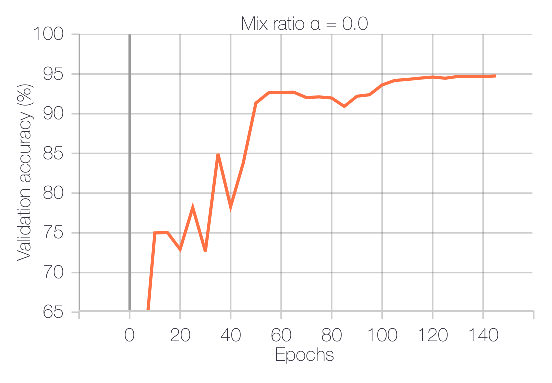
\includegraphics[width=0.48\textwidth]{figs/acc_loss_mix/mix0.0/nat_val_top1.eps}\\
    \vspace{10pt}
    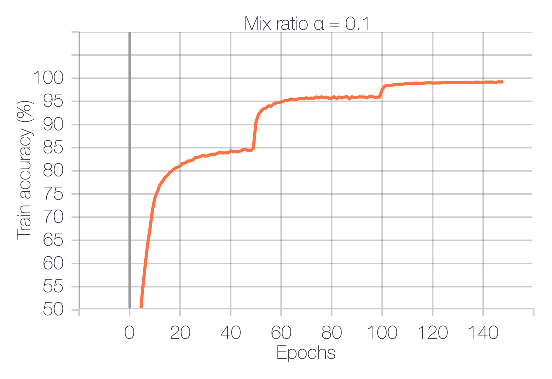
\includegraphics[width=0.48\textwidth]{figs/acc_loss_mix/mix0.1/nat_train_top1.eps}
    \hspace{10pt}
    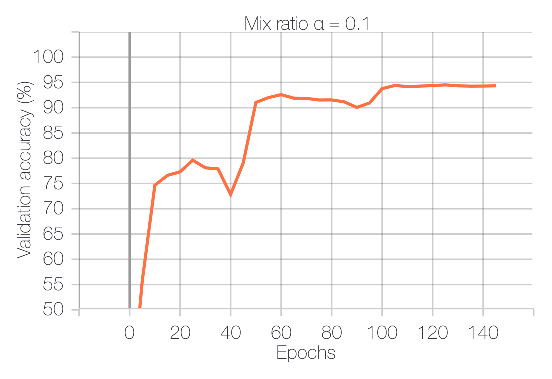
\includegraphics[width=0.48\textwidth]{figs/acc_loss_mix/mix0.1/nat_val_top1.eps}\\
    \vspace{10pt}
    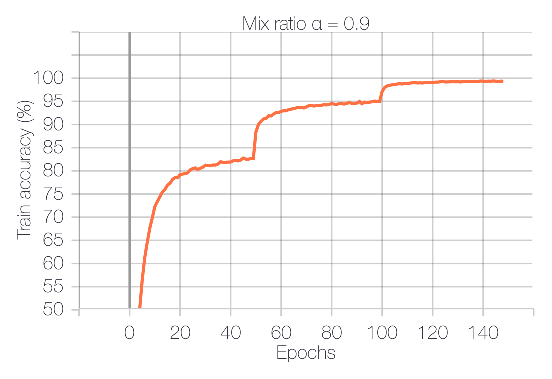
\includegraphics[width=0.48\textwidth]{figs/acc_loss_mix/mix0.9/nat_train_top1.eps}
    \hspace{10pt}
    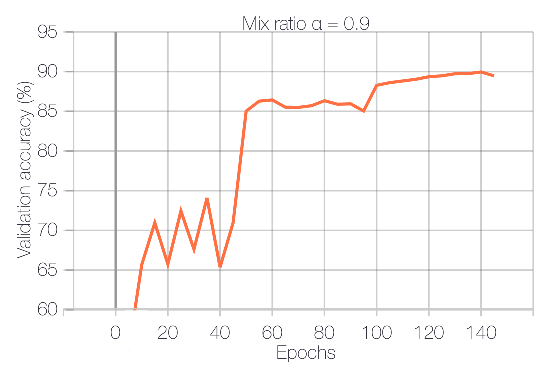
\includegraphics[width=0.48\textwidth]{figs/acc_loss_mix/mix0.9/nat_val_top1.eps}\\
    \vspace{10pt}
    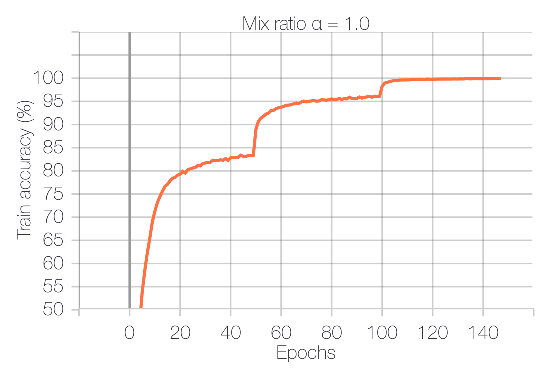
\includegraphics[width=0.48\textwidth]{figs/acc_loss_mix/mix1.0/nat_train_top1.eps}
    \hspace{10pt}
    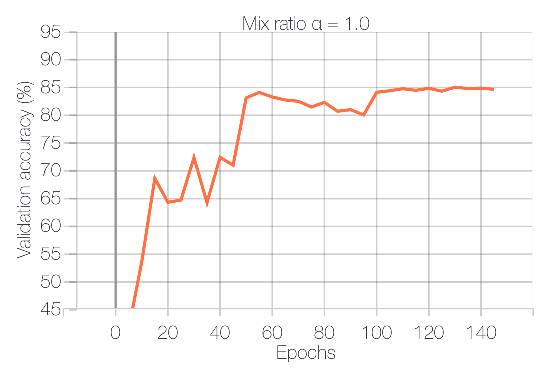
\includegraphics[width=0.48\textwidth]{figs/acc_loss_mix/mix1.0/nat_val_top1.eps}\\
\end{figure}

